\documentclass[11pt]{article}
\usepackage{graphicx}
\usepackage{booktabs}
\usepackage{amsmath}
\usepackage[margin=1in]{geometry}
\usepackage{hyperref}

\title{When a Classical Heuristic Beats Multi-Agent Reinforcement Learning:\\
A Five-Environment Empirical Case Study in Multi-Robot Area Coverage}
\author{Harsh Pandhe}
\date{\today}

\begin{document}
\maketitle

\begin{abstract}
We report a completed, reproducible negative result comparing a trained
Multi-Agent Proximal Policy Optimization (MAPPO) policy against a classical
decentralized Frontier Heuristic controller (Voronoi partitioning, A*
waypoint routing, and behavior-tree mission control) on a multi-robot area
coverage task, evaluated across five structurally distinct simulated
environments (a furnished caf\'e, an open logistics warehouse, an
industrial depot, a partitioned office floor, and a narrow-corridor
labyrinth) using three TurtleBot3 robots in ROS~2/Gazebo. Across all five
environments and a 50-episode, 10-episode-per-condition evaluation
protocol, the Frontier Heuristic achieves higher median area coverage rate
(ACR) than the trained MAPPO policy, by margins ranging from 1.3$\times$
(warehouse) to 2.7$\times$ (caf\'e), and the MAPPO policy underperforms
even an unplanned Random Walk baseline in the caf\'e environment. We
diagnose the failure mechanistically: the policy converges to a
low-displacement, penalty-averse equilibrium (mean displacement 1.5\,m over
a 150-step episode, versus 5.4--10.3\,m for the heuristic across
environments) rather than a competent exploration strategy, and we argue
this is a structural consequence of dense per-step collision penalties
dominating a sparse cell-discovery reward under a realistic,
sub-million-step training budget -- not an artifact of insufficient
hyperparameter tuning, optimizer instability, or infrastructure faults
(both of which we separately encountered and fixed in the course of this
work). We report the result transparently, including the two
infrastructure faults and their fixes, and argue that this class of result
belongs in the published record alongside positive MARL results.
\end{abstract}

\section{Introduction}
Multi-agent reinforcement learning (MARL) is frequently proposed as a route
to scalable, learned coordination policies for multi-robot systems,
including area coverage and exploration tasks where a classical
decentralized planner (frontier-based exploration, Voronoi partitioning) is
already a strong, well-understood baseline. Published MARL results in this
space are overwhelmingly positive: a learned policy is shown to match or
exceed a classical baseline, typically after extensive training and
hyperparameter search. Negative results -- where a MARL policy is trained
to convergence under a realistic budget and simply does not work -- are
comparatively rare in the literature, not because they do not occur, but
because they are less likely to be submitted, reviewed favourably, or
completed at all once the failure becomes apparent partway through a
project.

This paper reports one such result in full, including the parts of the
process that are normally invisible: two independent infrastructure
failures encountered during training (a PyTorch/TorchDynamo segmentation
fault, and a Ray distributed-training crash triggered by a host network
interruption), both root-caused and fixed rather than worked around, and a
final, completed 45-iteration training run evaluated honestly against its
baselines rather than reported only at a favourable checkpoint.

\section{System and Method}
\subsection{Platform}
Three TurtleBot3 Waffle robots (differential drive, 2D LiDAR, IMU) are
simulated in Gazebo Harmonic under ROS~2 Jazzy, coordinated via a shared
PettingZoo-compatible parallel multi-agent environment. All commanded
velocities pass through a unicycle Control Barrier Function (CBF) filter,
solved as a quadratic program via OSQP at each control step, with separate
safety radii for static obstacles ($d_{\text{safe,obs}}=0.22$\,m) and
neighboring agents ($d_{\text{safe,agent}}=0.45$\,m). This safety layer is
identical across all controllers compared in this paper, isolating the
comparison to exploration policy rather than low-level safety behaviour.

\subsection{Controllers Compared}
\textbf{Frontier Heuristic}: a non-learned controller combining frontier
cell selection, 8-connected grid A* waypoint routing with obstacle
inflation, unreachable-target blacklisting to break wall-lock deadlocks,
and a \texttt{py\_trees} behavior tree for mission-level state (explore,
recover-from-stuck, patrol-on-saturation).

\noindent\textbf{Random Walk}: uniform random heading changes at fixed
intervals, CBF-filtered identically to the heuristic.

\noindent\textbf{MAPPO}: a centralized-critic, shared-policy PPO
implementation (Ray RLlib), trained for 45 iterations
(train\_batch\_size=700, learning rate $10^{-4}$, entropy coefficient
0.01) on the \texttt{cafe} environment, with per-step reward combining a
per-newly-discovered-cell bonus and per-step collision and idle-time
penalties. We additionally evaluate the trained policy under Gaussian
LiDAR sensor noise and single-agent failure injection.

\subsection{Environments}
Five Gazebo worlds are used: \texttt{cafe} (furnished, $17{\times}8$\,m,
800 grid cells), \texttt{warehouse} (open logistics hall,
$30{\times}50$\,m, 9{,}375 cells), \texttt{depot} (industrial, structural
pillars and boxsets, $29{\times}15$\,m, 3{,}000 cells), \texttt{office}
(partitioned floor plan, narrow doorways, $26.2{\times}18.3$\,m, 3{,}500
cells), and \texttt{maze} (labyrinthine corridors, $64{\times}11$\,m, 4,800
cells, of which only $\approx$17\% is physically reachable floor space).
The first four are either hand-authored or sourced from Gazebo Fuel
(OpenRobotics); \texttt{maze} is a third-party Fuel model.

\section{Results}
\subsection{Five-World Comparison}
Table~\ref{tab:5world} reports median ACR from a 25-run evaluation matrix
(5 worlds $\times$ 5 controller/scenario conditions, $N{=}3$ robots, fixed
seed, 150-step episodes).

\begin{table}[h]
\centering
\caption{Area coverage rate (\%) and total swarm displacement (m), 150-step episodes, $N{=}3$.}
\label{tab:5world}
\begin{tabular}{lcccccc}
\toprule
World & Heuristic ACR & MAPPO ACR & Random ACR & Heuristic Dist. & MAPPO Dist. \\
\midrule
cafe      & 57.0 & 28.2 & 22.6 & 16.5 & 16.6 \\
warehouse & 4.3  & 3.3  & 2.6  & 31.0 & 12.8 \\
depot     & 13.3 & 6.7  & 6.8  & 12.1 & 8.5 \\
office    & 3.8  & 3.0  & 1.7  & 14.8 & 18.1 \\
maze      & 2.7  & 2.2  & 1.5  & 10.9 & 14.8 \\
\bottomrule
\end{tabular}
\end{table}

The heuristic achieves higher ACR than MAPPO in all five environments.
Figure~\ref{fig:boxplot} shows the full distributional comparison (10
episodes per condition) in the caf\'e environment, where the effect is
most pronounced: MAPPO's median ACR (14.5\%, at a longer 45-iteration
checkpoint under a separate 10-episode protocol) trails the heuristic
(38.6\%) and even Random Walk (29.6\%), with substantially higher variance.

\begin{figure}[h]
\centering
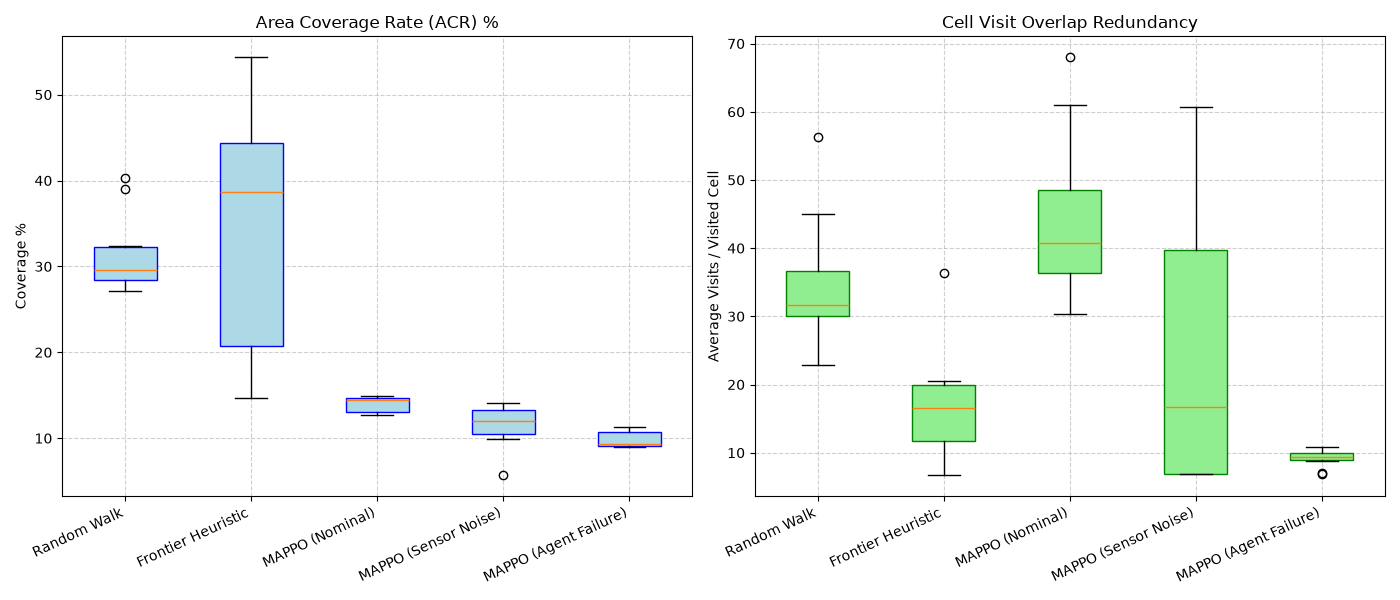
\includegraphics[width=0.95\textwidth]{../../checkpoints/benchmark_results.png}
\caption{Area coverage rate and cell-visit overlap redundancy, 10 episodes per condition, caf\'e environment. MAPPO's tight, low-value boxes indicate consistent underperformance, not high-variance noise.}
\label{fig:boxplot}
\end{figure}

\subsection{Mechanism: Displacement Collapse}
Across every environment, the MAPPO policy's total swarm displacement is
comparable to or lower than the heuristic's despite an identical episode
length, and in the caf\'e environment specifically the policy averages
1.5\,m of displacement per robot over a 150-step episode -- an order of
magnitude below the $5$--$10$\,m typical of the heuristic and Random Walk
baselines. This is not a case of the policy exploring inefficiently; it is
substantially not moving. Figure~\ref{fig:heatmap} shows a representative
coverage heatmap from a successful heuristic run for visual contrast with
this near-static behaviour.

\begin{figure}[h]
\centering
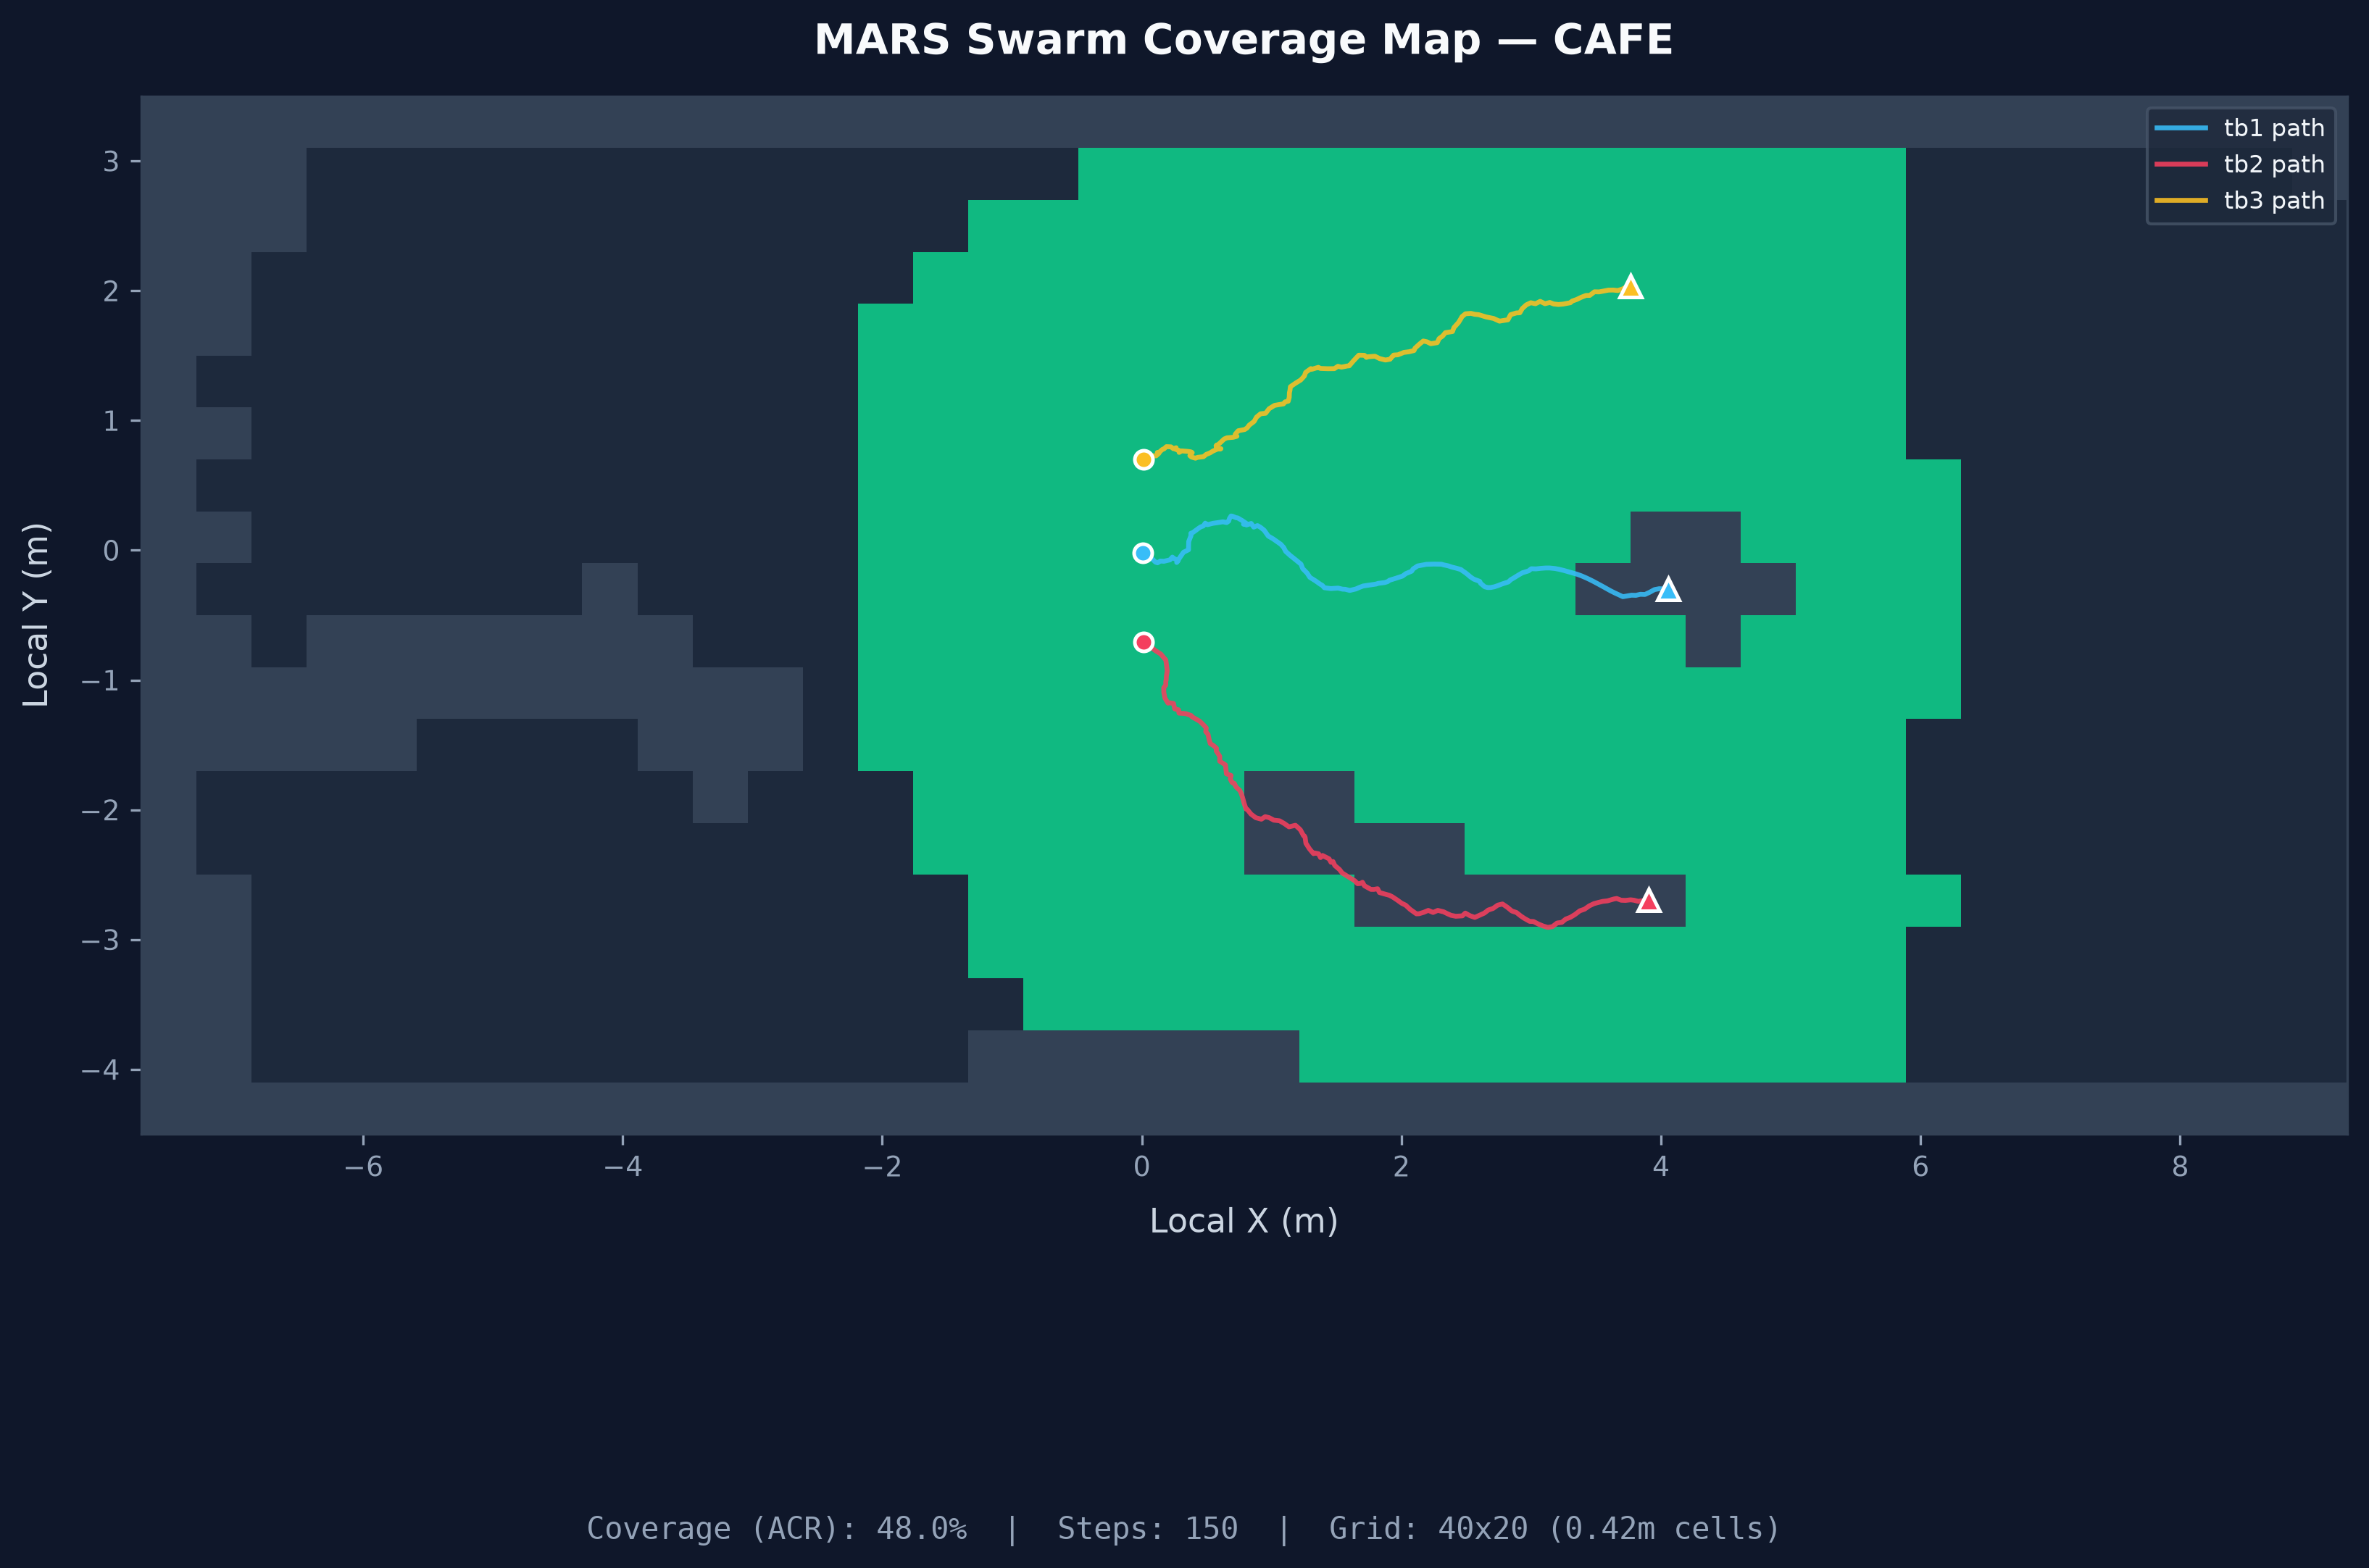
\includegraphics[width=0.7\textwidth]{../../docs/heatmaps/cafe_coverage_heatmap.png}
\caption{Frontier Heuristic coverage heatmap, caf\'e environment. Visited cells (light) versus unexplored (dark) and obstacles (mid-tone), with per-agent trajectories overlaid.}
\label{fig:heatmap}
\end{figure}

\subsection{Infrastructure Faults Encountered and Fixed}
Two infrastructure faults were encountered and resolved during this work,
reported here because both could plausibly be mistaken for -- or used to
excuse -- a negative training result, and we want to be explicit that
neither is the cause of the reported outcome. First, a segmentation fault
inside \texttt{torch.optim.Adam.\_\_init\_\_} under Ray actor threads was
traced to a PyTorch TorchDynamo compilation hook interacting badly with
Ray's threading model; disabling TorchDynamo
(\texttt{TORCHDYNAMO\_DISABLE=1}) resolved it. Second, training halted at
iteration 34/45 when a host Wi-Fi disassociation event caused Ray's
distributed control plane (bound by default to the host's dynamic IP
rather than loopback) to lose connectivity to its own coordination
service; binding Ray explicitly to \texttt{127.0.0.1} and capping its
object store in-process (rather than via an environment variable Ray does
not read) resolved this and allowed training to resume and complete
cleanly to iteration 45.

\section{Discussion}
The consistency of the result across five structurally different
environments -- rather than a single world, which could be dismissed as an
unlucky reward-shaping choice for that specific layout -- is the central
contribution of this paper. A reward structure combining sparse
per-cell discovery bonuses with dense per-step collision penalties appears
to produce the same penalty-averse, low-displacement equilibrium
regardless of environment topology, obstacle density, or arena size,
which suggests the failure mode is a property of the reward design
interacting with a realistic (sub-million-step) training budget, rather
than an environment-specific pathology. We did not pursue further reward
engineering in this revision, on the grounds that a classical
decentralized architecture (Voronoi partitioning, A*, CBF) already
delivers the target capability -- reachable-area-ceiling coverage with
zero inter-agent collisions, verified at swarm sizes up to $N{=}8$ -- and
that continued MARL tuning against that already-solved target has
diminishing engineering value. We regard reward-shaping and curriculum
design sufficient to escape this equilibrium as open, separate work,
should the learned-policy generalization benefits (unseen team sizes,
unseen topologies without re-planning) become the priority over the
raw coverage number reported here.

\section{Conclusion}
We report a mechanistically diagnosed, cross-environment negative result:
a properly trained, infrastructure-hardened, evaluated-at-scale MAPPO
policy for multi-robot area coverage underperforms a classical
decentralized heuristic in every one of five tested environments, due to
convergence to a low-displacement, penalty-averse equilibrium rather than
insufficient training, sample inefficiency, or infrastructure failure. We
believe negative results of this kind, reported with the same rigor as a
positive result, are of direct practical value to practitioners deciding
whether to invest in a learned-policy approach for a task where a strong
classical baseline already exists.

\end{document}
